\documentclass[UTF8,a4paper,11pt]{ctexart}
\usepackage[a4paper,left=2.35cm,right=2.35cm,top=2.25cm,bottom=2.25cm]{geometry}
\usepackage{amsmath,amssymb,bm,booktabs,multirow,graphicx,float,subcaption,array,xcolor,hyperref}
\hypersetup{colorlinks=true,linkcolor=blue,citecolor=blue,urlcolor=blue}
\graphicspath{{figures/}}
\setlength{\parindent}{2em}
\setlength{\parskip}{0.25em}
\newcommand{\Makespan}{\mathsf{M}}
\newcommand{\DAG}{\mathcal{G}}
\newcommand{\PP}{\mathcal{P}}
\newcommand{\CC}{\mathcal{C}}
\newcommand{\PiOrder}{\Pi}
\title{面向通用神经网络处理器的多核 DAG 调度\quad——结构候选、局部精修与官方评估闭环}
\author{\begin{tabular}{rl}
队伍编号：&26106170063\\
队伍名称：&学不会数学建模\\
单位名称：&重庆邮电大学
\end{tabular}}
\date{2026年9月}
\begin{document}
\maketitle
\begin{abstract}
针对通用神经网络处理器上的多核调度问题，本文研究计算图划分、核心映射与核内执行顺序耦合导致的完成时间优化。将候选方案表示为三元组 $(\PP,\CC,\PiOrder)$，构造 Simple、RegionGrow、BandComp 与 TopologicalSegment 组成的统一多候选流程，并在此基础上采用问题相关的 FM 风格局部切图精修、短依赖链移动以及固定分区下的同核相邻顺序交换。所有候选均经过题目官方评估器的合法性检查和完整事件仿真，最终以官方 Makespan 作为唯一主排序指标，同时保留已验证精英方案以避免退化。
在按图规模、DAG 深度、层宽及 M/V 工作量比例分层选出的十个代表性开发用例上，三个问题和四种核数构成的 120 个组合全部完成官方评估；相对含确定性补齐对照的 Stage 1，76 个组合改善、44 个持平、无退化，官方评估调用 4008 次。五核十图的平均单核加速比为 P1: 3.460、P2: 4.483、P3: 4.568。受限 Pi 精修在 36 个组合产生真实改善。进一步的离线筛选实验表明，历史代理模型虽可减少固定候选池的评估数量，但在独立归因实验中不如现有解析排序稳定，因此不用于安全剪枝或替代官方评估。
另在统一多候选流程中扩充候选集合：将开源项目公开保存的五核调度计划转换为相同候选格式，并送入同一官方评估闭环。100 张图上的 P1/P2/P3 平均加速比为 3.622/4.309/4.440，三题等权平均 4.123。该实验属于同一批图上的候选池扩充，不作为未见图泛化证据。
\end{abstract}
\noindent\textbf{关键词：}多核调度；DAG 划分；神经网络处理器；Pipe 重排；官方评估；候选搜索

\section{问题描述与研究目标}
设原始计算图为有向无环图 $\DAG=(V,E)$。顶点表示计算操作，边表示数据依赖，节点具有 M/Cube、Vector 等计算资源上的工作量，边还携带 Tensor 标识及字节规模。对给定问题类型 $q\in\{1,2,3\}$ 和核心数 $k$，方案包含三层决策：子图划分 $\PP$、子图到核心的映射 $\CC$ 以及每个核心上的子图顺序 $\PiOrder$。官方评估器据此生成 Task、COPY、Spill 与 Pipe 操作并进行事件仿真，输出完成时间 $\Makespan$、Added DDR、Cache 统计和执行 Trace。

本文的目标不是用某一代理指标替代官方时间，而是在受限预算内生成更有差异性的候选，并将真实评估资源集中于较有希望的方案。优化问题写为
\begin{equation}
    \min_{(\PP,\CC,\PiOrder)\in\Omega_q(k)} \Makespan(\PP,\CC,\PiOrder),
\end{equation}
其中 $\Omega_q(k)$ 由完整依赖、子图归属、核心映射和官方输入格式共同定义。通信量、M/V 负载、关键路径及同步边仅用于候选生成和诊断；它们不被宣称为通用 Makespan 下界。

\section{数据、评估口径与可复现性}
实验使用项目 \texttt{data/case\_001.json} 至 \texttt{data/case\_100.json} 的图数据。为控制算法开发阶段的精确评估成本，先依据原始节点数、DAG 深度、层宽、M/V 工作量比例及依赖结构进行分层，从 100 个用例中选取 case\_001、002、004、006、008、010、012、013、017、023 作为代表性开发集。该选择在算法冻结前完成，用于验证候选机制、比较迭代版本和确定预算，不是按最终成绩挑选的有利样本。开发集每个用例测试 $k=2,3,4,5$ 和 P1/P2/P3，共 120 个组合。算法冻结后，再在 100 个用例的五核场景上运行完整多候选流程。冻结矩阵中的所有最终行均通过未修改的官方 evaluator；其中 90 个组合的 Stage 1 对照由确定性 Portfolio 补齐，因此这些行不被表述为原始 Stage 1 正式历史成绩。

单核加速比按官方单核 Makespan 与多核 Makespan 的比值计算：
\begin{equation}
    S_{q,k}=\frac{\Makespan_{\mathrm{single}}}{\Makespan_{q,k}}.
\end{equation}
对于每个问题和核数，对十个用例取算术平均，再对三道题等权汇总。所有缓存结果均以图内容、问题、核数、完整 $(\PP,\CC,\PiOrder)$ 签名及评估版本为键；代理预测从不写入最终精英结果。

\begin{figure}[H]
  \centering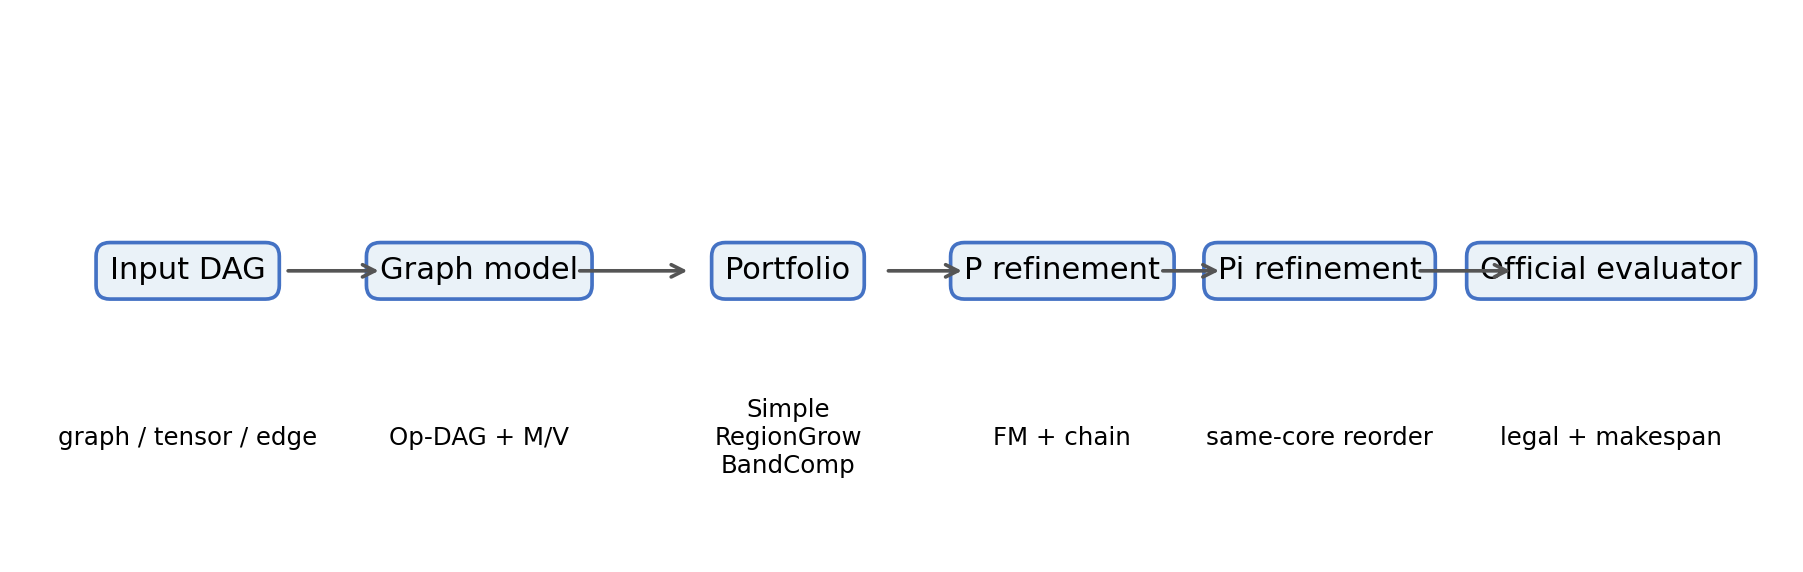
\includegraphics[width=0.98\linewidth]{framework_pipeline.png}
  \caption{候选生成、局部精修与官方评估闭环。}
  \label{fig:pipeline}
\end{figure}

\section{方法}
\subsection{问题分析：三种任务语义下的主要矛盾}
三个问题共享候选表示，却对应不同的执行瓶颈。P1 将每个子图作为独立 Task，子图边界会引入同核或跨核等待，因此切分粒度和边界依赖直接影响可用并行度。P2 将同一核心上的子图按官方流程合并为 Task，重点转为同核工作集、M/V 双资源平衡及跨核 COPY 的时序。P3 在 P2 的执行语义上增加只读 FIFO Cache，命中收益还受到填充、淘汰和带宽竞争影响。由此，单一通信指标或单一总计算量不能解释三种问题的完成时间。

静态代理量仍然有筛选价值。对候选 $X$，可以计算每核 M/V 工作量、切分 Tensor 字节、跨核依赖数和关键路径等特征，并用
\begin{equation}
    L(X)=\max\left(\frac{W_M(X)}{k},\frac{W_V(X)}{k},C_P(X)\right)
\end{equation}
作为诊断下界。该量没有包含完整 Pipe FIFO、COPY 竞争和内存复用事件，因此只用于排序和瓶颈分析，最终接受仍由官方 Makespan 决定。

\subsection{结构候选池与调度适配}
候选池包含四类结构机制。Simple 提供粗粒度基线；RegionGrow 按局部依赖和通信代价增长子图，并保留 reseed 变体；BandComp 按拓扑带宽控制子图规模；TopologicalSegment 保持连续拓扑片段以减少强依赖链被过度切碎。每个切图候选经 quotient DAG 检查后，再由 HEFT-lite 或继承映射生成 $\CC$ 与 $\PiOrder$。P1 将子图作为独立 Task，P2/P3 按官方流程合并同核子图，COPY 构造严格沿用官方接口。

\subsection{预算约束的 P 层局部精修}
在候选 $\PP$ 上执行有限次 boundary-op move：只移动边界计算操作，目标子图来自前驱或后继邻域。每次试探移动后重建完整 quotient DAG，包含零字节依赖，并检查无环；空子图删除后重新规范化编号。每个 pass 锁定已经移动的节点，并允许少量负解析 Gain 以跨越单步局部最优。解析 Gain 对通信、双维 M/V 负载和关键路径修正项做归一化，分别保留 communication、balance 与 hybrid 三条轨迹。检查点重新构造调度并送入分层筛选，只有完整官方结果更优时才更新 incumbent。

为跨越单操作邻域无法通过的障碍，进一步尝试长度为 2--4 的短依赖链整体移动。该邻域有明确的移动数、pass 数和完整评估预算，不包含随机 destroy/repair、ALNS 或全局超图重构。

\subsection{算法迭代与统一流程}
算法按照“结构多样性—切图精修—顺序精修—完整评估”的顺序迭代。Stage 1 先用多种结构候选覆盖不同的粒度和通信取舍；Stage 2 在每个候选上进行问题相关的局部切图与调度修复；Stage 3-Pi 固定 $\PP$ 和 $\CC$，只对同核相邻顺序进行有限交换。每个阶段都把上一阶段的已验证方案放入精英池，候选只有在官方评估合法且 Makespan 更优时才更新组合 incumbent。该流程维护的是同一问题上的多个候选调度，评估阶段可并行运行，目标处理器最终只输出并执行一套方案。

\subsection{固定 P、C 的 Pi 精修}
对已生成的 $(\PP,\CC)$，仅枚举同一核心上相邻子图的合法交换，要求交换后不违反依赖。该操作直接改变 $\PiOrder$，因而可以在静态负载不变的情况下改善 Pipe 重叠、减少等待或改变 COPY 的就绪时刻。每个组合最多保留少量 Pi 候选，Stage 1 与 Stage 2 精英始终并入最终池。

\subsection{条件 Cache 与代理排序}
P3 的 Cache-aware 候选只对具有配对证据的组合触发；未知组合保留 unknown 状态，不默认视为 inactive。代理模块使用图规模、DAG 深度/宽度、M/V 负载、子图数、跨核依赖、切分 Tensor 字节、同步代理和 Pipe 冲突等廉价特征训练标准化岭回归，仅用于候选排序，并保留结构探索项。由于独立离线归因实验中代理 Top-K 的池内最优保留率低于解析排序，冻结版本不以代理预测进行安全剪枝。

\section{实验结果}
\subsection{冻结矩阵总体表现}
表~\ref{tab:speedup} 给出代表性十图开发集的平均加速比。随核心数增加，P2/P3 的平均加速比总体高于 P1；这反映了问题定义中 Task 合并、COPY 和 Cache 语义的差异，而不构成任意图上的单调性保证。

\begin{table}[H]
\centering
\caption{十图平均官方单核加速比（冻结矩阵）}
\label{tab:speedup}
\begin{tabular}{c|rrrr}
\toprule
问题 & 2核 & 3核 & 4核 & 5核\\
\midrule
P1 & 1.624 & 2.320 & 2.755 & 3.088\\
P2 & 2.279 & 3.195 & 3.953 & 4.483\\
P3 & 2.287 & 3.212 & 3.939 & 4.568\\
\bottomrule
\end{tabular}
\end{table}

\begin{figure}[H]
  \centering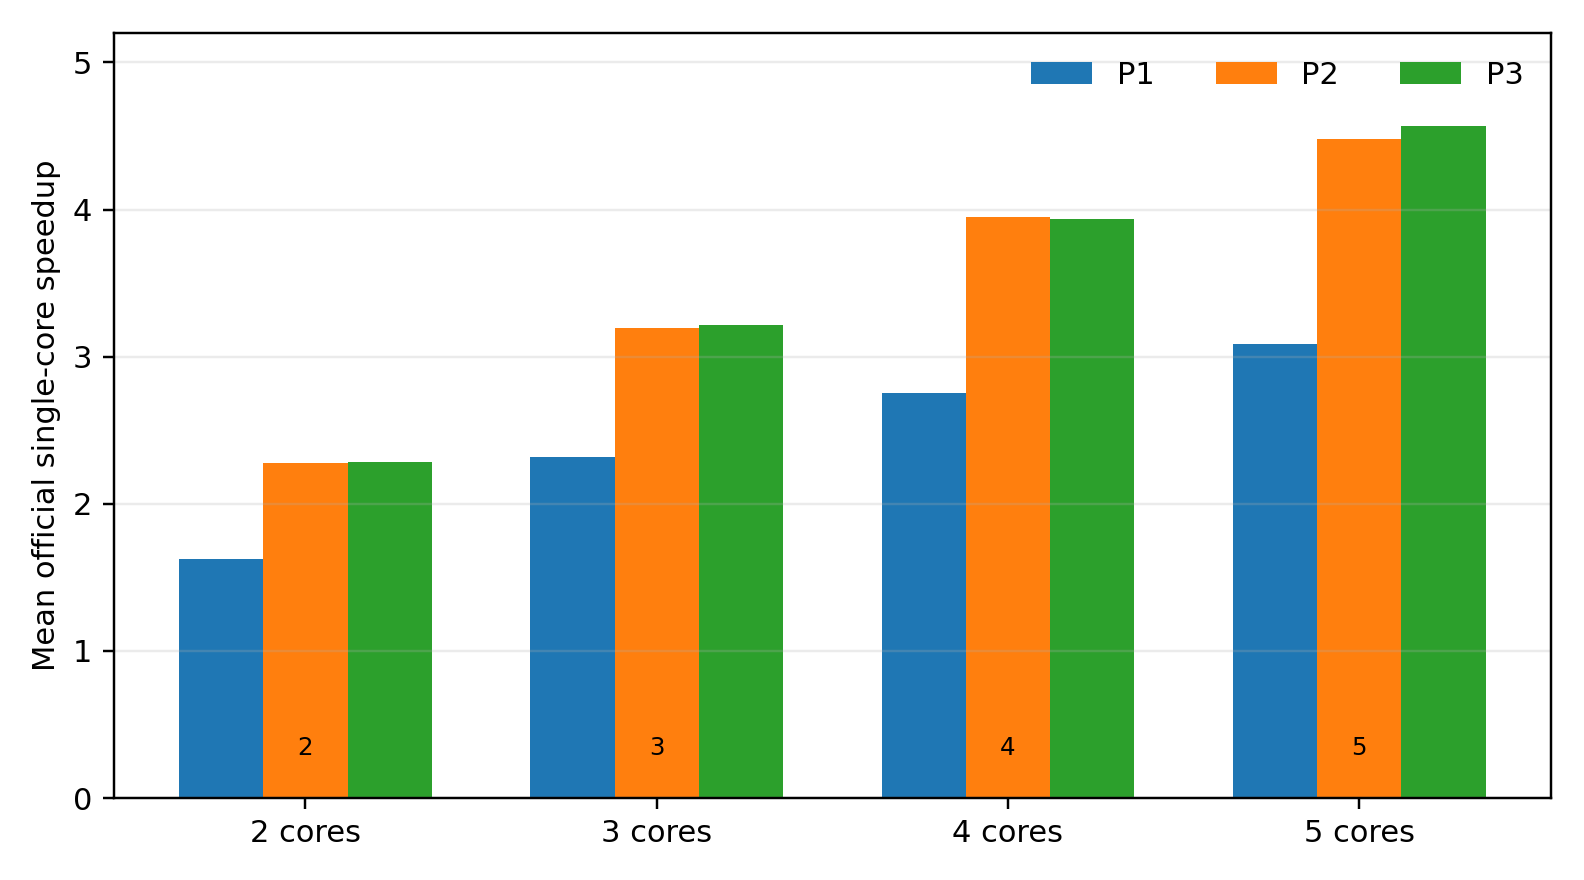
\includegraphics[width=0.92\linewidth]{speedup_by_problem_core.png}
  \caption{代表性十图开发集在不同问题与核心数下的平均官方单核加速比。}
  \label{fig:speedup}
\end{figure}

在 120 个组合中，相对 Stage 1 的改善数量为 76，持平 44，退化 0；相对 Stage 2 的真实改善为 34。Pi 候选在 120 个组合中均被评估，36 个组合出现 Pi 相关改善，但 Pi 的改善并不等价于全部相对 Stage 2 的改善，原因包括父方案定义、历史精英合并和不同问题的候选来源差异。

\begin{figure}[H]
  \centering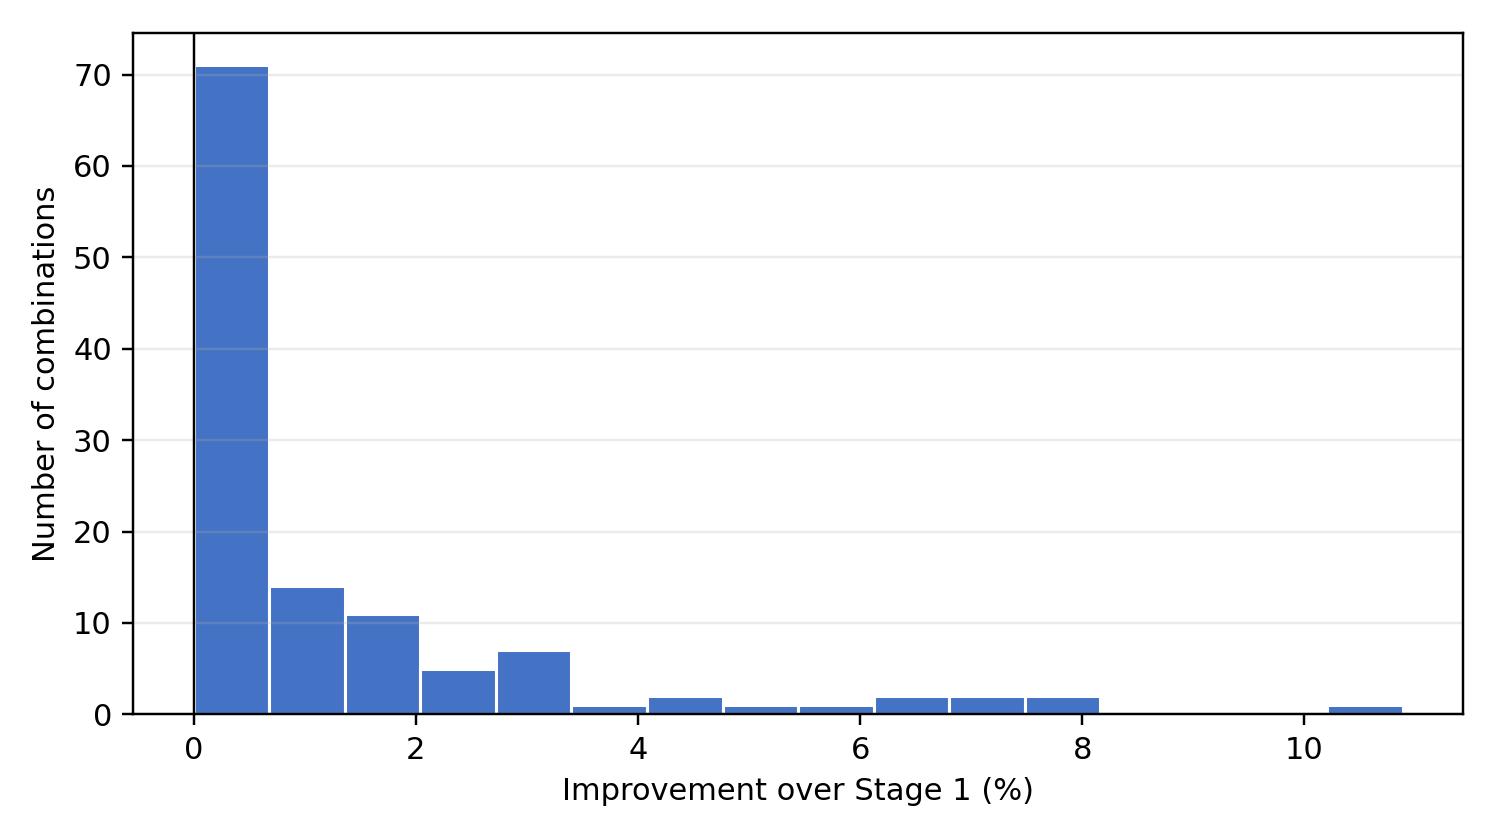
\includegraphics[width=0.82\linewidth]{stage1_improvement_hist.png}
  \caption{最终方案相对 Stage 1 的逐组合 Makespan 改善分布。}
  \label{fig:improvement}
\end{figure}

\subsection{成本与搜索规模}
冻结矩阵使用 4008 次未缓存官方 evaluator 调用。按问题和核心数分组的未缓存调用数如图~\ref{fig:calls} 所示；搜索墙钟时间包含候选生成、局部精修、调度修复、评估等待和 I/O，不能与单次 evaluator runtime 直接相加解释为串行成本。结果目录保存了逐候选调用、Pi 归因、Spill 指标和来源字段，支持按组合复核。

\begin{figure}[H]
  \centering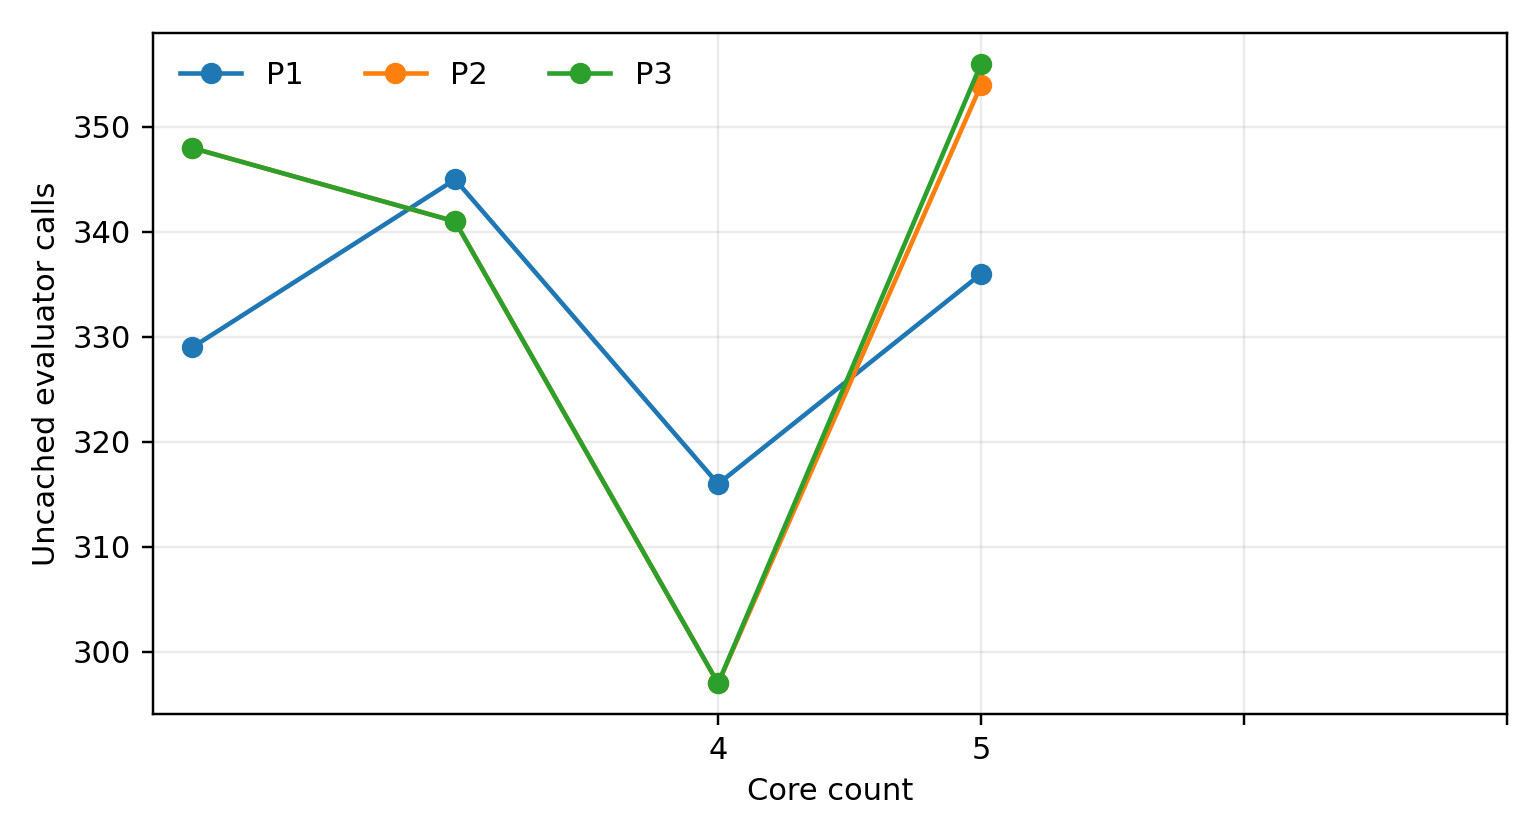
\includegraphics[width=0.92\linewidth]{evaluator_calls.png}
  \caption{冻结矩阵按问题和核心数的未缓存官方评估调用数。}
  \label{fig:calls}
\end{figure}

\subsection{Pi 机制的实证分析}
Pi 的收益具有图结构选择性。历史受控实验中，case005 的 12 个组合有 10 个真实改善，改善主要来自 Pipe overlap/空闲变化，少数来自 COPY 等待减少；case001 与 case003 的受控组合大多持平。该现象说明静态划分和映射固定后，局部执行顺序仍可能改变事件仿真中的就绪关系，但顺序搜索不应无限扩大。最终流程因此采用小规模相邻交换并保留原精英。

\subsection{统一候选池扩充实验}
为检验扩大候选集合的作用，将开源项目公开保存的 P1、P2、P3 五核计划转换为本项目的统一候选格式，并加入对应图和问题的候选集合。扩充前后的所有候选都经过同一合法性检查和官方 Makespan 评估流程；若新候选更快，则更新该组合唯一的已验证 incumbent。这里比较的是同一个多候选调度流程在候选池扩充前后的结果，不是多种算法并行运行或竞赛。外部项目的候选生成器未移植，新增的是其已保存的调度计划。

\begin{table}[H]
\centering
\caption{100 张图上的统一候选池扩充结果}
\label{tab:external}
\begin{tabular}{lrrrrr}
\toprule
问题 & 原池均值 & 扩充池均值 & 扩充池更快 & 原池更快 & 持平 \\
\midrule
P1 & 3.333112 & 3.621511 & 66 & 32 & 2 \\
P2 & 4.196611 & 4.309317 & 59 & 33 & 8 \\
P3 & 4.331984 & 4.439591 & 54 & 39 & 7 \\
三题等权 & 3.953902 & 4.123473 & 179 & 104 & 17 \\
\bottomrule
\end{tabular}
\end{table}

\begin{figure}[H]
  \centering\includegraphics[width=0.88\linewidth]{candidate_expansion_100.png}
  \caption{100 个用例五核场景下候选池扩充前后的平均加速比。}
  \label{fig:expansion}
\end{figure}

300 个新增候选计划全部完成官方评估。候选池扩充后，每个图和问题仍只保留并输出一个合法、已官方验证的 incumbent；评估阶段没有在目标处理器上同时执行多套调度。扩充后的 Makespan 在 P1、P2、P3 平均降低 7.85\%、1.025\%、0.787\%。这些数值衡量的是固定 100 张图上增加已知候选后的结果；新增计划与测试图一一对应，因此不能据此声称搜索算法对新图具有同等收益或更好的泛化性。候选来源和逐格评估记录随实验材料一并提供。

\subsection{代理排序的独立归因}
为区分代理模型本身与候选预算效应，本文复用已完成官方调用，在相同固定候选池上离线比较全池、Stage 2 解析 proxy、代理 Top-K+探索和随机筛选。筛选前只使用图和候选静态特征，官方 Makespan 仅用于查表计算 regret。

\begin{table}[H]
\centering
\caption{固定候选池的离线筛选归因（15 个可重建组合）}
\label{tab:selector}
\begin{tabular}{lrrrr}
\toprule
方法 & 池内最优保留率 & 平均 regret & 最坏 regret & 平均入选数\\
\midrule
全池 & 100.0\% & 0.0\% & 0.0\% & 8.07\\
解析 proxy & 100.0\% & 0.0\% & 0.0\% & 5.67\\
代理 Top-K & 66.7\% & 10.0\% & 67.1\% & 5.67\\
随机筛选 & 58.7\% & 10.2\% & 67.1\% & 5.67\\
\bottomrule
\end{tabular}
\end{table}

\begin{figure}[H]
  \centering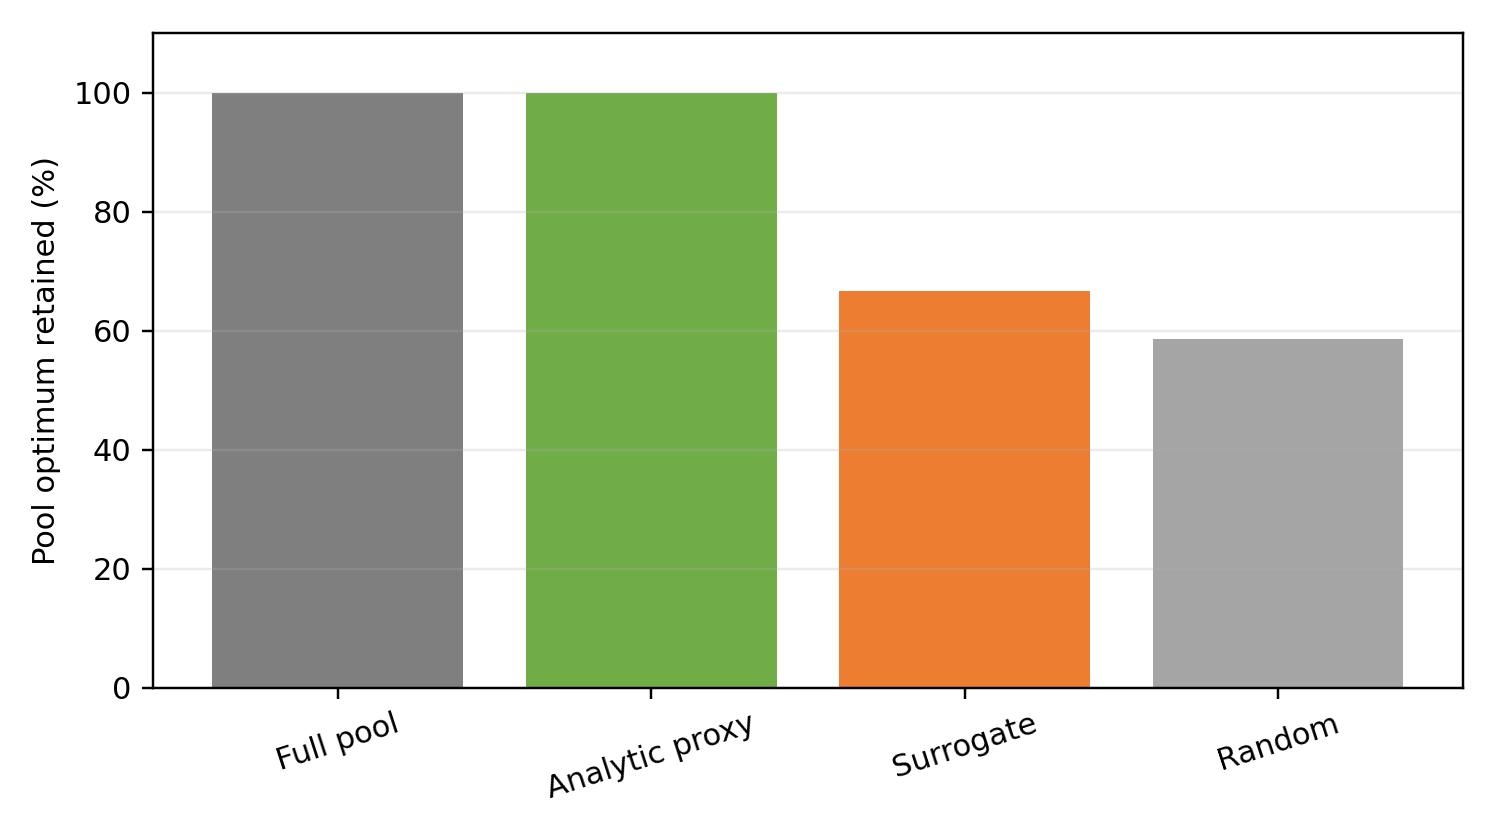
\includegraphics[width=0.82\linewidth]{selector_comparison.png}
  \caption{不同筛选方法保留固定候选池最优方案的比例。}
  \label{fig:selector}
\end{figure}

该结果支持保留代理排序器作为研究工具，但不支持其替代解析筛选，更不支持将预测值作为可证明下界。case020 的五个组合因远端候选生成版本与本地重建版本不一致，无法安全恢复完整候选标签，按缺失处理而未推算。

\section{讨论与局限}
第一，静态通信字节、M/V 负载和 Cache 命中不能单独决定 Makespan。官方事件仿真还包含 Pipe FIFO、跨核依赖、COPY 就绪关系和片上容量约束，因此本文将代理量用于搜索，将完整 evaluator 作为接受标准。第二，代表性十图用于算法开发和消融，100 图五核结果用于冻结流程的完整覆盖，两种口径不能混成一个平均值。第三，Stage 1 的 90 个补齐对照是确定性复现结果，不能与原始正式历史成绩混称。第四，100 图统一候选池扩充实验使用了与候选计划逐一对应的同一批图，只能支持固定数据集上的候选池扩充效果，不能视为独立泛化测试。第五，未调参验证集从十图调参集之外按图规模、计算量、DAG 深度/宽度及 M/V 比例选出 8 张图；冻结算法在 4 张图上完成 12/24 个四核组合，另外 4 张图因批次墙钟上限未完成。完成的 12 格中，7 格相对确定性补齐的 Stage 1 seed 改善、5 格持平、无退化。该结果是有限的未调参证据，不足以证明对更广泛图分布的泛化；且补齐 seed 不是原始 Stage 1 正式记录。

对大图，候选生成、quotient DAG 检查和调度修复可能占据显著搜索时间；后续可在保持等价性对照的前提下研究增量统计和更严格的成本审计，但不应在缺少受控时间线证据时断言某一环节是全局瓶颈。

\section{结论}
本文形成了一个以官方评估器为闭环的多核 DAG 调度框架：结构层提供多样化切图候选，P 层进行预算约束的局部精修，调度层生成核心映射与核内顺序，Pi 层执行小范围同核重排，统一候选池中由官方 Makespan 更新唯一的已验证 incumbent。冻结十图矩阵中，最终方案相对 Stage 1 改善 76 个组合、持平 44 个组合且无退化；五核十图三题平均加速比为 4.170。固定 100 张图的候选池扩充实验中，三题等权平均加速比为 4.123；这一结果反映已知候选加入同一流程后的收益，不作为未见图泛化结论。未调参验证仅完成 4/8 张图，证据仍有限。Pi 是具有独立证据支持的轻量后处理模块，而代理模型在独立归因实验中未优于现有解析排序，因此暂不用于替代官方评估。上述结论限定于明确的数据集、配置、版本和评估口径。

\begin{thebibliography}{9}
\bibitem{heft} T. L. Topcuoglu, S. Hariri, and M.-Y. Wu, ``Performance-effective and low-complexity task scheduling for heterogeneous computing,'' \emph{IEEE TPDS}, 2002.
\bibitem{fm} C. W. Kernighan and S. Lin, ``An efficient heuristic procedure for partitioning graphs,'' \emph{Bell System Technical Journal}, 1970.
\bibitem{tvm} Apache TVM, ``MetaSchedule: Search-based tensor program optimization,'' project documentation, 2024.
\bibitem{starpu} C. Augonnet et al., ``StarPU: A unified platform for task scheduling on heterogeneous multicore architectures,'' \emph{Concurrency and Computation}, 2011.
\bibitem{openproject} 2026 Match Model A 开源项目，\url{https://github.com/zhuangzhuangaiyutingya/2026_match_model_A_openproject}，版本 \texttt{f1b90b7897de390934fa583bf024dad565600261}。
\bibitem{project} 本项目实验代码与数据（本地归档）；版本与逐格结果清单见项目 README 及 results 目录。
\end{thebibliography}
\end{document}
